\documentclass[11pt,a4paper]{article}
\usepackage[margin=2.2cm]{geometry}
\usepackage[T1]{fontenc}
\usepackage{mathpazo}
\usepackage{textcomp}
\usepackage{microtype}
\usepackage{graphicx}
\usepackage{booktabs}
\usepackage[font=small,labelfont=bf]{caption}
\usepackage{titlesec}
\usepackage{xcolor}
\usepackage[hidelinks]{hyperref}
\urlstyle{same}

% House style: no hyphens or dashes anywhere in the text.
\hyphenpenalty=10000
\exhyphenpenalty=10000
\emergencystretch=3em
\newcommand{\m}{\textminus}
\newcommand{\uV}{\textmu V}

\titleformat{\section}{\large\bfseries}{\thesection}{0.8em}{}
\titleformat{\subsection}{\normalsize\bfseries}{\thesubsection}{0.8em}{}
\setlength{\parskip}{0.35em}
\linespread{1.03}

\title{\textbf{The Song or the Self?}\\[0.3em]
\large A preregistered search for personal musical emotion in scalp EEG}
\author{Aditya Koundinya\\
\small Independent researcher, Bengaluru, India\\
\small aditya003koundinya@gmail.com}
\date{October 2026}

\begin{document}
\maketitle

\begin{abstract}
\noindent Twenty people can hear the same song and walk away feeling twenty different things. If the brain carries a signature of emotion, it should follow what each listener actually felt, not only what the song was designed to make them feel. This study asked whether scalp EEG tracks that personal part of musical emotion. Using the public MET Music Induced EEG Dataset (20 listeners, 20 two minute excerpts each, 66 channel EEG), I tested three preregistered hypotheses: that a listener who felt more aroused than usual would show lower posterior alpha power (H1), that a listener who felt more pleasant than usual would show relatively greater left frontal activity, indexed by frontal alpha asymmetry (H2), and that the strength of these links would differ between people (H3). Each rating was also split into the part shared by all listeners (the song consensus) and the part unique to the person (the personal deviation). After quality control, 395 trials entered linear mixed models. None of the hypotheses was supported. The within person arousal slope on posterior alpha was 0.05 standardized units (95\% CI \m0.05 to 0.15, $p = .355$), opposite in sign to the prediction; the valence slope on frontal asymmetry was 0.01 (95\% CI \m0.10 to 0.11, $p = .903$); the person specific deviation slopes were equally small; and random slope variances were estimated at essentially zero. A grid of 105 exploratory tests yielded nothing that survived correction, and the result held across four alternative analyses and when each listener was left out in turn. Because the confidence intervals are narrow, they rule out more than they confirm: a one standard deviation shift in a person's felt arousal is unlikely to lower their posterior alpha by more than about 0.05 standard deviations. I argue that classic alpha markers of emotion, measured over whole songs, are too coarse to see the personal side of musical feeling.
\end{abstract}

\section{Introduction}

\subsection{A puzzle about the same song}

Put on a piece of music in a room full of people and watch their faces. Some will brighten, some will drift, and one person may be quietly moved by a melody that leaves everyone else unaffected. Music is one of the most reliable everyday sources of emotion, and it produces strong feelings even though nothing is at stake for the listener. Juslin and V\"astfj\"all (2008) argued that this happens through a family of mechanisms, from simple reflexes to the sheer energy of a sound, to expectation, memory and personal association. Some of these mechanisms belong to the song: a fast, loud, bright passage raises arousal in almost anyone. Others belong to the listener: the song that played at a friend's wedding or during a hard year carries a meaning no one else hears.

This creates a puzzle for anyone who wants to find emotion in the brain. When we compare a cheerful song with a sad one, the brain responses differ, but so do the tempo, the loudness, the timbre and a hundred other acoustic features. The brain may simply be responding to the sound. The cleanest test of whether the brain tracks \emph{feeling}, rather than the stimulus, is to hold the song constant and ask whether a person who felt more than others did also shows a different brain response. That is the question this paper sets out to answer.

\subsection{Two old ideas about emotion in the EEG}

Psychologists often describe emotion along two broad dimensions: valence, which runs from unpleasant to pleasant, and arousal, which runs from calm to excited (Russell, 1980). These dimensions can be measured quickly with the Self Assessment Manikin, a pictorial scale on which a person marks how they feel after a stimulus (Bradley \& Lang, 1994).

Scalp electroencephalography (EEG) records the summed electrical activity of large populations of cortical neurons. It has excellent timing but blurry spatial resolution, and it cannot see deep structures such as the amygdala that are central to emotion. EEG therefore never measures emotion directly. What it can offer are rhythms, and two rhythms have been proposed as windows onto the two emotional dimensions.

The first is \textbf{alpha power}, the 8 to 13 Hz rhythm that dominates the back of the head when a person is relaxed. Alpha power falls when the cortex becomes more engaged and alert (Klimesch, 1999; Barry et al., 2007). If feeling excited means being more cortically activated, then a more arousing experience should come with lower posterior alpha.

The second is \textbf{frontal alpha asymmetry} (FAA), the difference in alpha power between the right and left frontal cortex. Because alpha is inversely related to activity, relatively lower alpha on the left implies relatively greater left frontal activity, which has been linked to approach motivation and positive affect (Davidson, 1992; Coan \& Allen, 2004). Music studies have reported exactly this pattern, with greater left frontal activity for joyful and happy excerpts than for fearful and sad ones (Schmidt \& Trainor, 2001). At the same time, the FAA literature has a mixed replication record and is sensitive to choices such as the reference electrode (Allen, Coan, \& Nazarian, 2004; Reznik \& Allen, 2018).

\subsection{The hidden problem: whose emotion is it?}

Most of the evidence for these markers comes from comparing conditions: happy against sad songs, pleasant against dissonant music, positive against negative film clips. Such comparisons cannot separate the feeling from the stimulus that caused it. A second, quieter problem is statistical. A typical dataset contains many trials from each of a few people. If those trials are analysed as if they were independent, the analysis behaves as though it had hundreds of participants when it really has twenty, a mistake known as pseudoreplication (Hurlbert, 1984). The usual cure is a mixed model that treats people as the units of replication (Barr, Levy, Scheepers, \& Tily, 2013; Bates, M\"achler, Bolker, \& Walker, 2015).

This study tackles both problems together. Instead of comparing songs, it compares each listener with themselves: did a person whose rating of a song was higher than their own average also show a different EEG? And instead of trusting the raw rating, it splits every rating into two parts: what the other listeners felt about that song (the song consensus), and how far this listener departed from them (the personal deviation). The deviation is the purest available measure of the personal side of the experience, because it is, by construction, not shared with anyone else who heard the same sound.

\subsection{The plan, written down before the answer}

A study that searches through many brain measures will almost always find something by chance. To avoid fooling myself, I wrote down the hypotheses, outcome measures, exclusion rules, models and decision thresholds in a preregistration and committed it to version control on 6 October 2026, before any analysis relating EEG to ratings was run (Nosek, Ebersole, DeHaven, \& Mellor, 2018). The research question was:

\begin{quote}
\emph{Within individuals, is self reported emotional experience (valence and arousal) during two minute music excerpts associated with EEG band power, and does any association persist for the person specific part of the experience, beyond what is shared across listeners for the same song?}
\end{quote}

Three hypotheses followed from the literature above.
\textbf{H1:} higher within person arousal is associated with lower posterior alpha power.
\textbf{H2:} higher within person valence is associated with greater relative left frontal activity, that is, higher FAA.
\textbf{H3:} the within person slopes of H1 and H2 vary between participants.

\section{Method}

\subsection{The dataset}

I used the MET Music Induced EEG Dataset, version 1.0.4, published on OpenNeuro (Cheang, 2026). Twenty adults (aged 21 to 29; ten women and ten men) each listened to the same 20 songs, four from each of five intended categories: high valence and high arousal (HVHA, happy and energetic), high valence and low arousal (HVLA, pleasant and calm), low valence and high arousal (LVHA, tense), low valence and low arousal (LVLA, sad), and neutral. Each recording lasts about 131 seconds: roughly 5 seconds of silence, 120 seconds of music, then silence. After each song, listeners rated valence and arousal on 1 to 9 scales and liking and familiarity on 1 to 5 scales. EEG was recorded from 66 channels plus EOG at 1000 Hz and was distributed already preprocessed. This study used only the public data; no new data were collected.

\subsection{Opening the box}

Before any modelling, I inspected a single recording in detail, and then every file. The data did not always match their description. The files are in EEGLAB format rather than BrainVision as the dataset documentation states; amplitudes are in microvolts although the channel table lists volts; flat channels are labelled ``good''; and the spectra show a sharp dip at 50 Hz, revealing a notch filter that is not documented. Recordings also carry no marker for music onset, so the music window was assumed from the documentation to run from 5 to 125 seconds. One recording (participant 12, song t05) is truncated in the published files at 62\% of its length, and one (participant 17, song t17) is missing entirely. Finally, acquisition timestamps repeat across files, so the order in which songs were played cannot be recovered. None of these issues could be fixed, but all of them were recorded, because each one limits what the data can show.

The inherited preprocessing included a 0.5 to 70 Hz band pass filter, the 50 Hz notch and an average reference. The frontal electrodes Fp1 and Fp2 barely correlated with the EOG channel ($r \approx \m0.09$), which suggests that blink artifacts had already been removed upstream, although no record of that step is stored. I deliberately did not filter, re reference or run independent component analysis again, so that my own choices would be few and transparent.

\subsection{Cleaning and measurement}

Within the music window, channels were flagged if they were flat (standard deviation below 0.5~\uV) or if their log standard deviation was extreme relative to the other channels (robust $|z| > 3$, using the median and median absolute deviation). Flagged channels were set to missing rather than interpolated. Each recording was cut into sixty non overlapping two second epochs. Epochs were dropped if they overlapped a segment annotated as bad in the dataset or if any remaining channel exceeded $\pm$100~\uV. Trials with fewer than 30 clean epochs (one minute of data) were excluded.

For each clean epoch, a Hann tapered Fourier transform gave a power spectrum, and these were averaged across epochs (the Welch method; Welch, 1967), giving a resolution of 0.5 Hz. Band power was the area under the spectrum in the delta (1 to 4 Hz), theta (4 to 8 Hz), alpha (8 to 13 Hz), beta (13 to 30 Hz) and gamma (30 to 45 Hz) bands, transformed to log10. The H1 outcome, \emph{posterior alpha}, was the mean log10 alpha power over O1, O2, Oz, PO3, PO4, POz and Pz. The H2 outcome, \emph{FAA}, was $\ln(\alpha_{F4}) \m \ln(\alpha_{F3})$, so that higher values mean relatively less alpha, and so more activity, on the left.

Table~\ref{tab:qc} traces every trial from the 400 possible listener and song pairs to the 395 that were analysed. Recordings were very clean overall: the median recording kept 59 of 60 epochs. Of the 213 recordings with at least one flagged channel, most flags fell on edge electrodes (F9, F10, T10), and only 12 touched the channels used for H1 or H2.

\begin{table}[!htb]
\centering
\caption{From 400 possible trials to 395 analysed trials.}
\label{tab:qc}
\small
\begin{tabular}{lrp{7.2cm}}
\toprule
Stage & Count & Reason for loss \\
\midrule
Listener and song pairs in the design & 400 & \\
EEG recordings present & 399 & participant 17, song t17 missing from the dataset \\
Recordings passing EEG quality control & 396 & participant 12, song t05 truncated; \\
 & & participant 14, song t06 only 26 clean epochs; \\
 & & participant 18, song t17 no clean epochs \\
Trials analysed & 395 & participant 01, song t27 missing liking and familiarity \\
\bottomrule
\end{tabular}
\end{table}

\subsection{Splitting each rating into song and self}

Every rating was decomposed in two ways. For the main tests, it was split into a \emph{within person} part (the rating minus that person's own average, which asks whether this song felt more than usual \emph{for them}) and a \emph{between person} part (the person's average minus the grand average). Only the within person part tests the hypotheses; the between person part is reported descriptively.

For the second half of the research question, the rating was split into a \emph{song consensus} and a \emph{personal deviation}. The consensus was the average rating that the other 19 listeners gave the same song (a leave one out mean, so that a person's own rating never enters their consensus). The deviation was the person's rating minus that consensus, centred within person. A positive arousal deviation means ``this song excited me more than it excited everyone else''.

\subsection{Statistical models}

H1 and H2 were tested with linear mixed models fitted in lme4 (Bates et al., 2015) with restricted maximum likelihood and Satterthwaite degrees of freedom from lmerTest (Kuznetsova, Brockhoff, \& Christensen, 2017). Each model predicted the EEG outcome from the within and between person rating, with a random intercept and a random within person slope for each participant, following the advice to keep the random structure maximal (Barr et al., 2013). If that structure was singular, the preregistered fallback first removed the correlation between the random intercept and slope, and then removed the random slope. A hypothesis was supported only if the slope had the predicted sign and $p < .025$, a Bonferroni correction across H1 and H2. Effects were standardized by multiplying the slope by the within person standard deviation of the rating and dividing by the within person standard deviation of the outcome.

The consensus and deviation models added song as a crossed random effect, to absorb whatever all listeners shared because of the music itself. The deviation slope is the person specific test; the consensus slope is descriptive only, because the consensus is a property of the song and so moves together with every acoustic feature that could alter the EEG directly. H3 compared the random slope model with the random intercept model using a likelihood ratio test. Because a variance cannot be negative, the test statistic does not follow an ordinary chi square distribution, and its $p$ value was taken from a 50:50 mixture of $\chi^2(1)$ and $\chi^2(2)$ (Self \& Liang, 1987).

\subsection{Exploratory and sensitivity analyses}

Beyond the confirmatory tests, a labelled exploratory grid crossed five bands, seven scalp regions and three ratings (valence, arousal and liking), for 105 models, corrected with the Benjamini and Hochberg false discovery rate (Benjamini \& Hochberg, 1995). Gamma results were flagged as vulnerable to muscle activity (Muthukumaraswamy, 2013). The confirmatory models were then refitted under four alternative choices: both ratings in one model; adding liking and familiarity; relative rather than absolute power; and a stricter $\pm$75~\uV{} threshold. Each was also refitted twenty times, leaving out one listener at a time. A preregistered check of presentation order could not be run, because the play order is not recoverable.

\section{Results}

\subsection{Did the songs do their job?}

Before asking about the brain, we need to know whether the songs moved people at all. Figure~\ref{fig:songs} places each song at its average rating. Arousal worked well: energetic and calm songs separated cleanly, from about 1.6 to 7.8 on the nine point scale. Valence worked less well. No song averaged below 3.1, so the intended ``negative'' songs were at most mildly unpleasant, and the neutral songs were mildly positive and calm. Valence and arousal were only weakly related (Spearman $\rho \approx 0.19$ pooled; mean within person $\rho = 0.18$), so H1 and H2 do test different aspects of experience.

\begin{figure}[!htb]
\centering
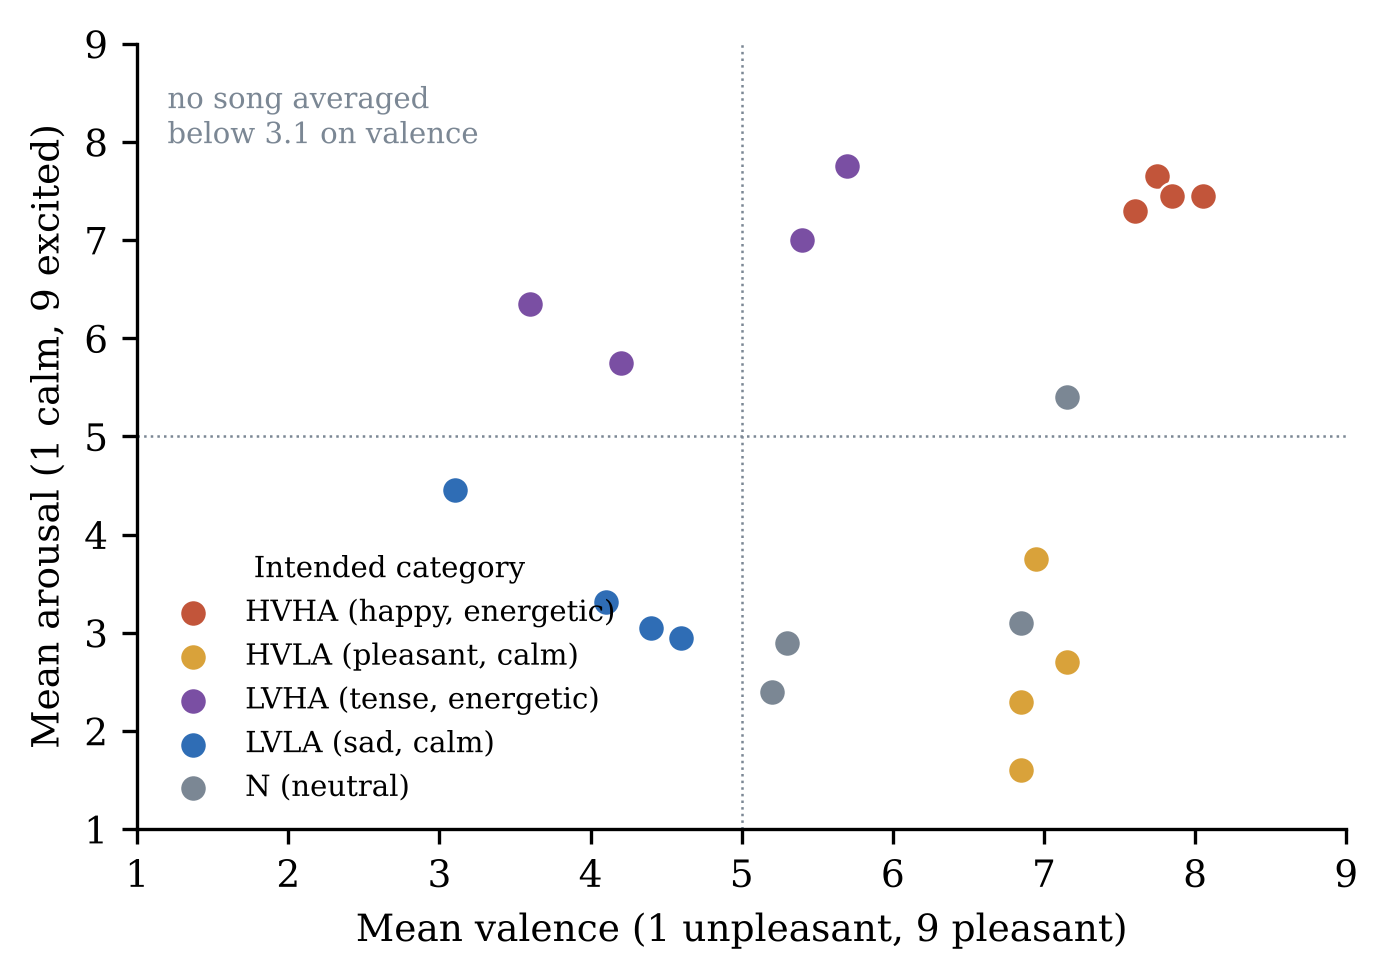
\includegraphics[width=0.6\linewidth]{figures/fig1_song_map.png}
\caption{Each dot is one song at its average rating across the 20 listeners, coloured by its intended category. Arousal spreads across nearly the whole scale; valence is compressed at the unpleasant end.}
\label{fig:songs}
\end{figure}

A crossed random effects model then asked where the variation in ratings came from. The song explained 49\% of the variance in valence and 67\% in arousal. A person's general rating habit explained only about 4\% of each. The remainder, the personal reaction to a particular song together with rating noise, was 47\% for valence and 29\% for arousal. Ratings, in other words, are mostly about the music, which confirms how much an ordinary between song comparison would be entangled with acoustics. But a large personal component remains, especially for valence, which leaves real room for the question this study asks.

\subsection{Does the measuring tool work?}

A null result is only meaningful if the instrument could have detected something. The pipeline passed three checks. It recovered a synthetic 10 Hz sine wave at exactly the right frequency and power. The spectra had the expected shape, falling with frequency and peaking near 10 Hz over the back of the head. And, as shown in Figure~\ref{fig:alpha}, alpha power was strongest over posterior regions, which is one of the most reliable findings in all of EEG research.

\begin{figure}[!htb]
\centering
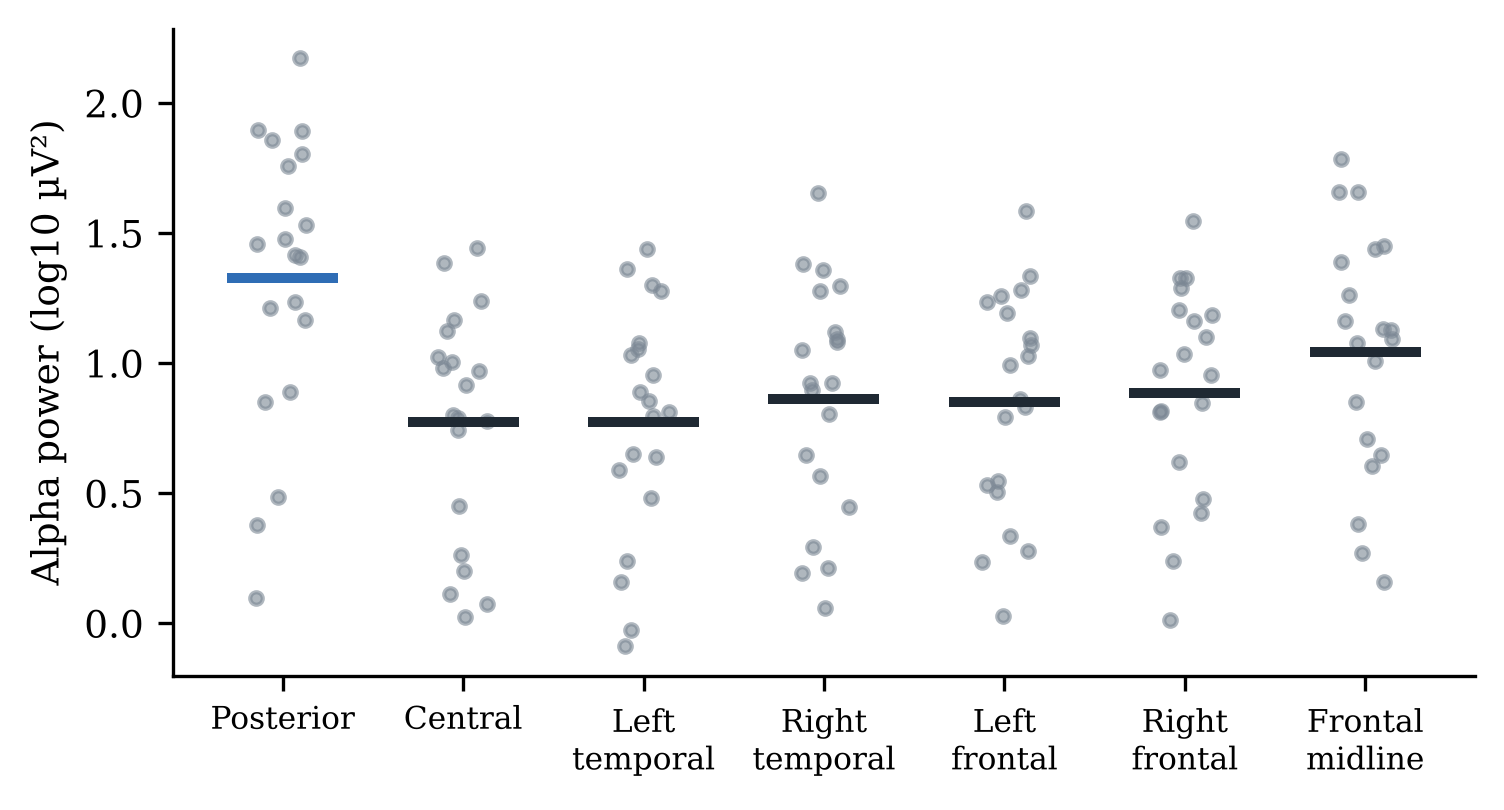
\includegraphics[width=0.66\linewidth]{figures/fig2_alpha_by_region.png}
\caption{Average alpha power in each scalp region. Grey dots are the 20 listeners; bars are the group means. Alpha is highest posteriorly, as expected, which supports the pipeline. Note how widely listeners differ from one another.}
\label{fig:alpha}
\end{figure}

Figure~\ref{fig:alpha} also previews the central difficulty. The grey dots, one per listener, are spread over a range of about two log units. About 94\% of the variance in posterior alpha lay between people, and only about 6\% varied from song to song within a person. Any emotional effect within a person had to show itself in that thin 6\% slice.

\subsection{A lesson in counting}

To make the pseudoreplication problem concrete, I ran the same H1 question three ways (Figure~\ref{fig:pool}). Treating all 395 trials as independent gave a correlation of 0.009 with a deceptively narrow confidence interval. Analysing each person separately and then combining the 20 individual correlations (the correct unit) gave 0.08 with a wider interval, from \m0.07 to 0.22. Correlating the 20 personal averages answered a different question entirely and gave an interval spanning almost half the possible range. None of the three found an effect. The point of the exercise is not the size of the estimate but the honesty of the interval: the naive analysis claims a precision the data do not have.

\begin{figure}[!htb]
\centering
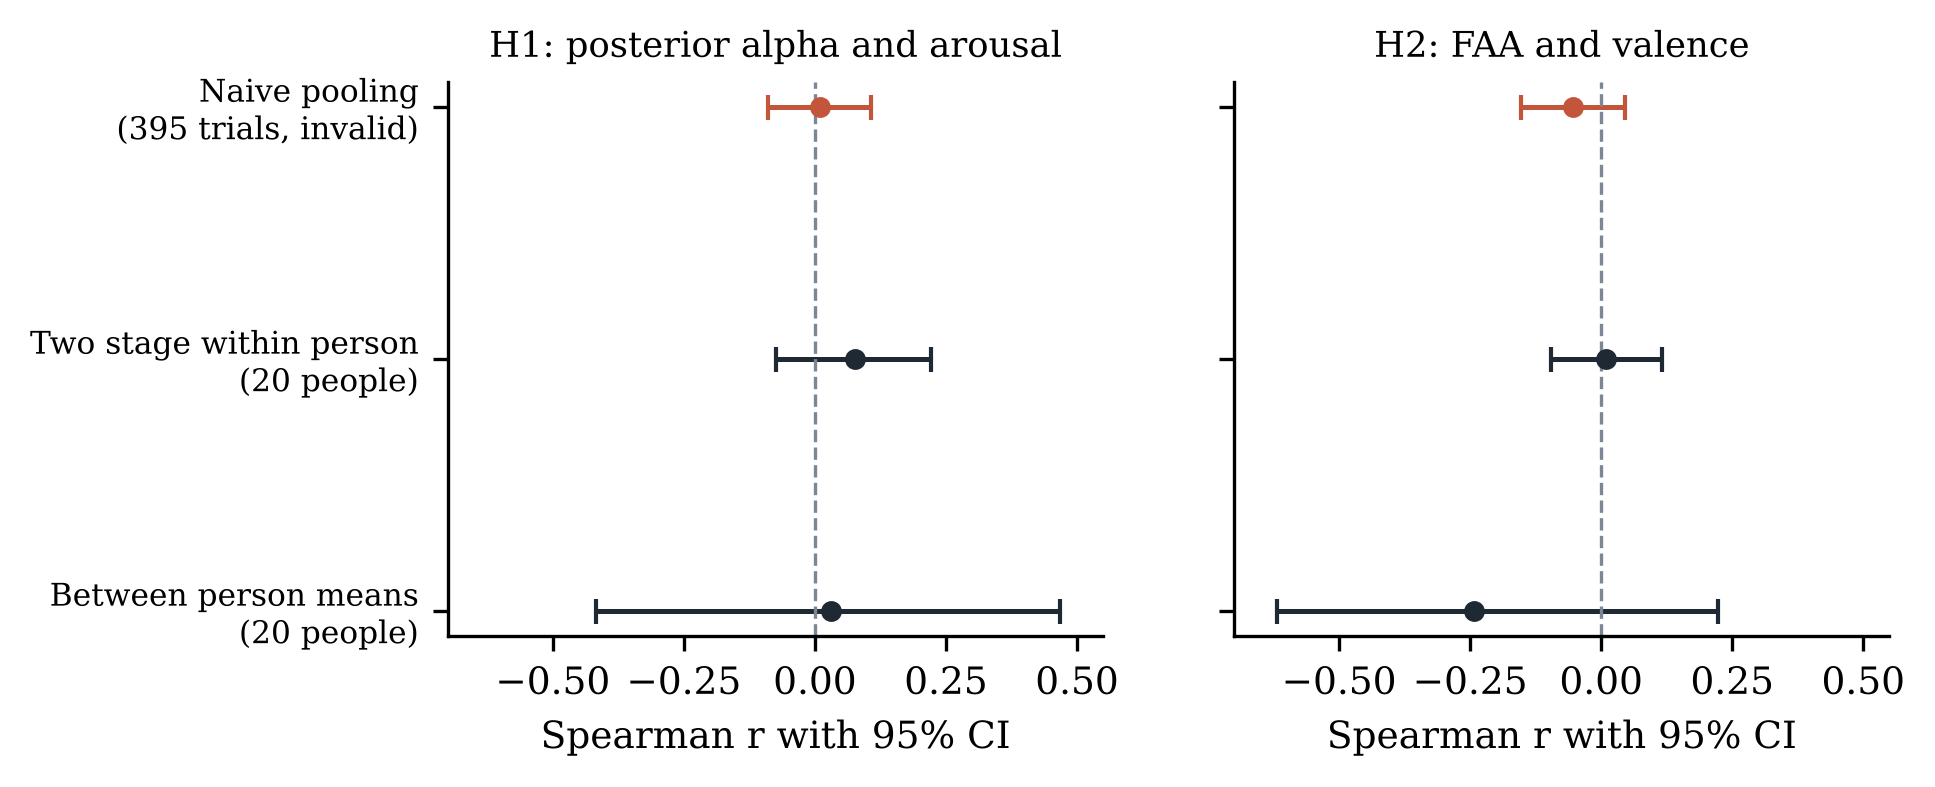
\includegraphics[width=0.82\linewidth]{figures/fig3_pooling.png}
\caption{The same question answered three ways. Naive pooling (orange) treats trials as independent and reports an interval that is too narrow. The two stage analysis treats the 20 people as the units.}
\label{fig:pool}
\end{figure}

\subsection{The confirmatory tests}

For both H1 and H2, the random slope structure was singular, so the preregistered fallback reduced each model to random intercepts only. Table~\ref{tab:main} and Figure~\ref{fig:forest} show the results.

\textbf{H1 was not supported.} A listener who felt more aroused than usual did not show lower posterior alpha. The standardized slope was 0.05 (95\% CI \m0.05 to 0.15, $p = .355$), and its sign was \emph{opposite} to the prediction: if anything, alpha was very slightly higher on more arousing songs.

\textbf{H2 was not supported.} A listener who felt more pleasant than usual did not show greater left frontal activity. The standardized slope was 0.01 (95\% CI \m0.10 to 0.11, $p = .903$), almost exactly zero.

\begin{table}[!htb]
\centering
\caption{Confirmatory results. Estimates are standardized within person slopes with 95\% profile confidence intervals. H1 and H2 used $\alpha = .025$; H3 used $\alpha = .05$.}
\label{tab:main}
\small
\begin{tabular}{llrcr}
\toprule
Test & Prediction & Estimate & 95\% CI & $p$ \\
\midrule
H1: arousal and posterior alpha & negative & 0.05 & [\m0.05, 0.15] & .355 \\
H2: valence and FAA & positive & 0.01 & [\m0.10, 0.11] & .903 \\
H1 person specific: arousal deviation & negative & 0.05 & [\m0.05, 0.15] & .342 \\
H2 person specific: valence deviation & positive & 0.04 & [\m0.06, 0.15] & .386 \\
H3 for H1: slopes differ between people & SD $> 0$ & SD $\approx$ 0.000 & not estimable & .949 \\
H3 for H2: slopes differ between people & SD $> 0$ & SD $=$ 0.006 & not estimable & .424 \\
\bottomrule
\end{tabular}
\end{table}

\begin{figure}[!htb]
\centering
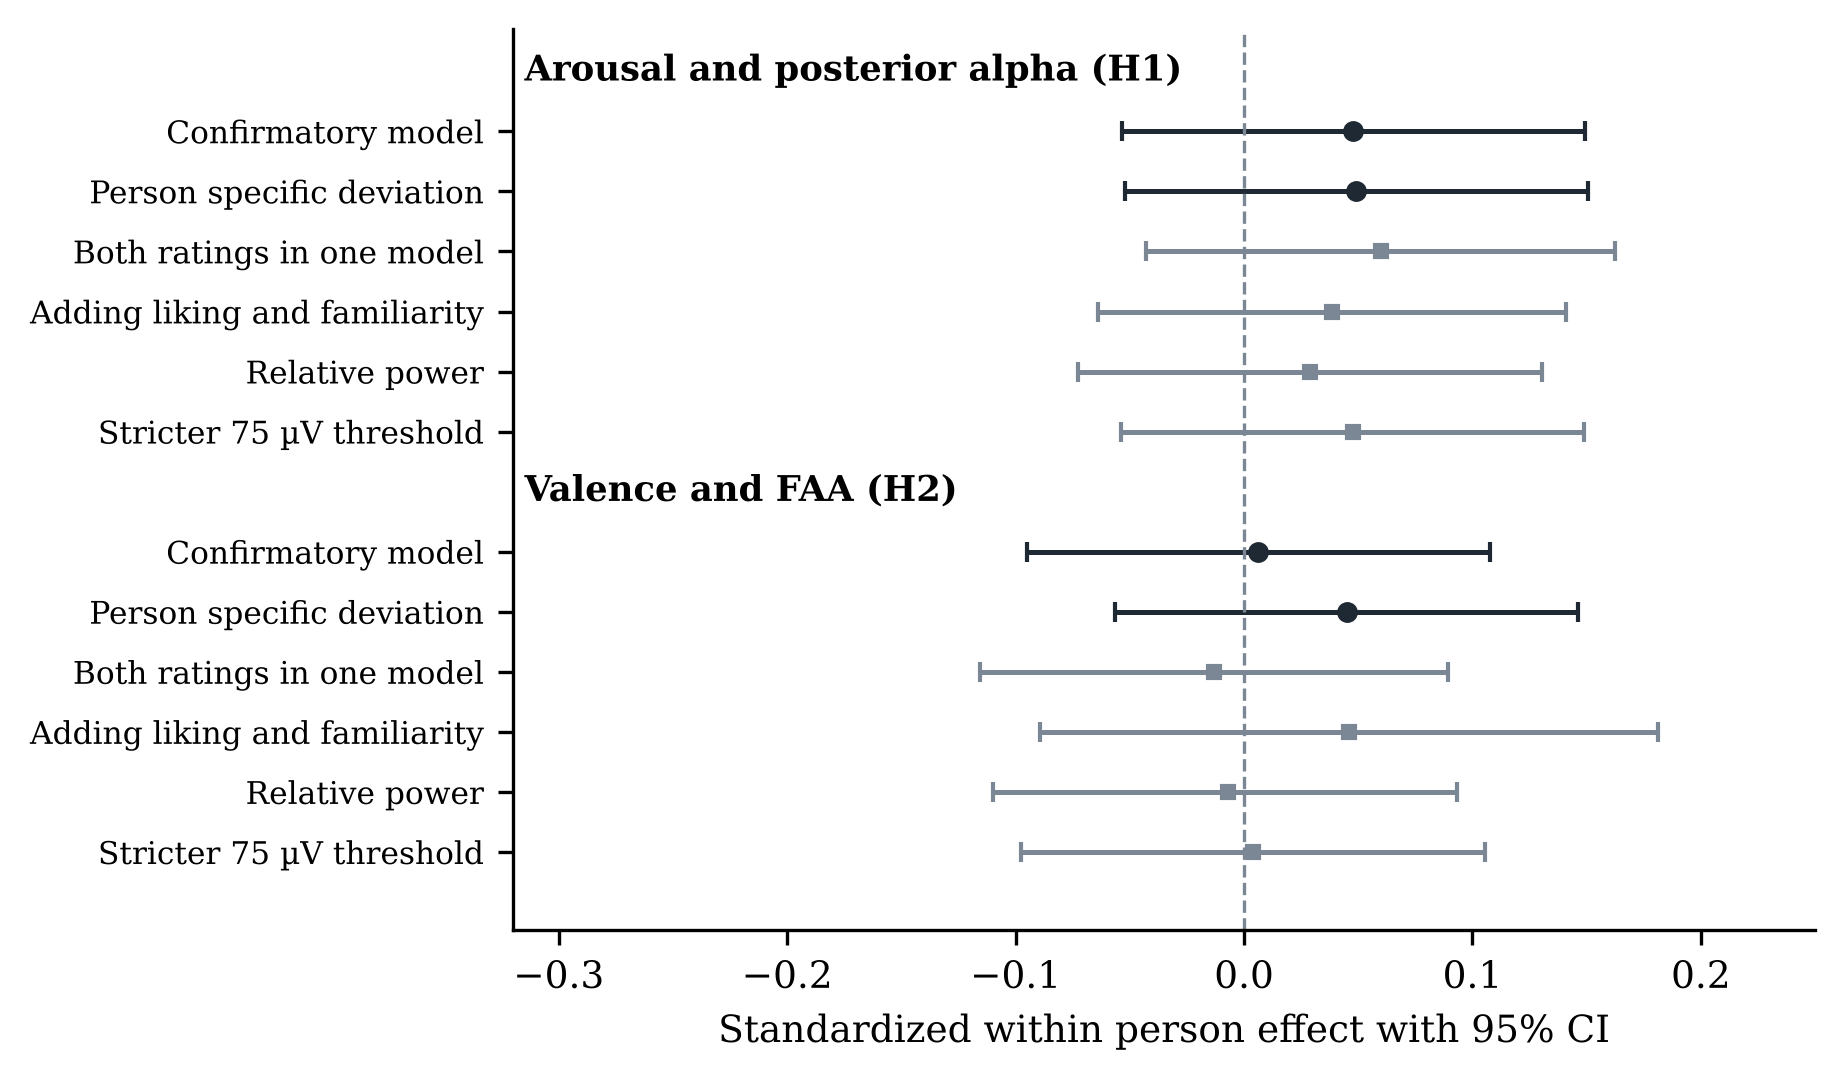
\includegraphics[width=0.66\linewidth]{figures/fig4_confirmatory.png}
\caption{Every estimate of the two main effects. Black circles are the confirmatory and person specific tests; grey squares are the four sensitivity analyses. All intervals cross zero and all sit close to it.}
\label{fig:forest}
\end{figure}

\subsection{Song versus self}

The second half of the research question asked about the personal part of the experience. Here, too, the answer was null. When a listener found a song more arousing than the other listeners did, their posterior alpha did not change detectably (standardized 0.05, 95\% CI \m0.05 to 0.15, $p = .342$). When a listener found a song more pleasant than the others did, their frontal asymmetry did not change either (0.04, 95\% CI \m0.06 to 0.15, $p = .386$). The song consensus slopes were also near zero ($p = .625$ for arousal and $p = .507$ for valence), but these could not have been read as emotion effects in any case, because the consensus is bound up with the acoustics of each song. In the valence model, the variance attributable to songs was itself close to zero, a further sign that frontal asymmetry was not following the music in any systematic way.

\subsection{Are people different?}

It is tempting to imagine that the effect exists but runs in opposite directions in different people, cancelling out on average. H3 tested this directly. Figure~\ref{fig:slopes} shows each listener's raw slope for H1. At first glance they look different: some point down, some point up. But each slope rests on only about 20 songs, and its interval is wide. The mixed model, which weighs each person's slope by its reliability, estimated the true spread at essentially zero for H1 (SD $\approx$ 0.000; likelihood ratio 0.01, mixture $p = .949$) and close to zero for H2 (SD $=$ 0.006; likelihood ratio 1.15, $p = .424$). Both random slope models were singular, so intervals for these spreads could not be estimated. The apparent individual differences are what noise looks like when each person contributes only 20 data points. H3 was not supported.

\begin{figure}[!htb]
\centering
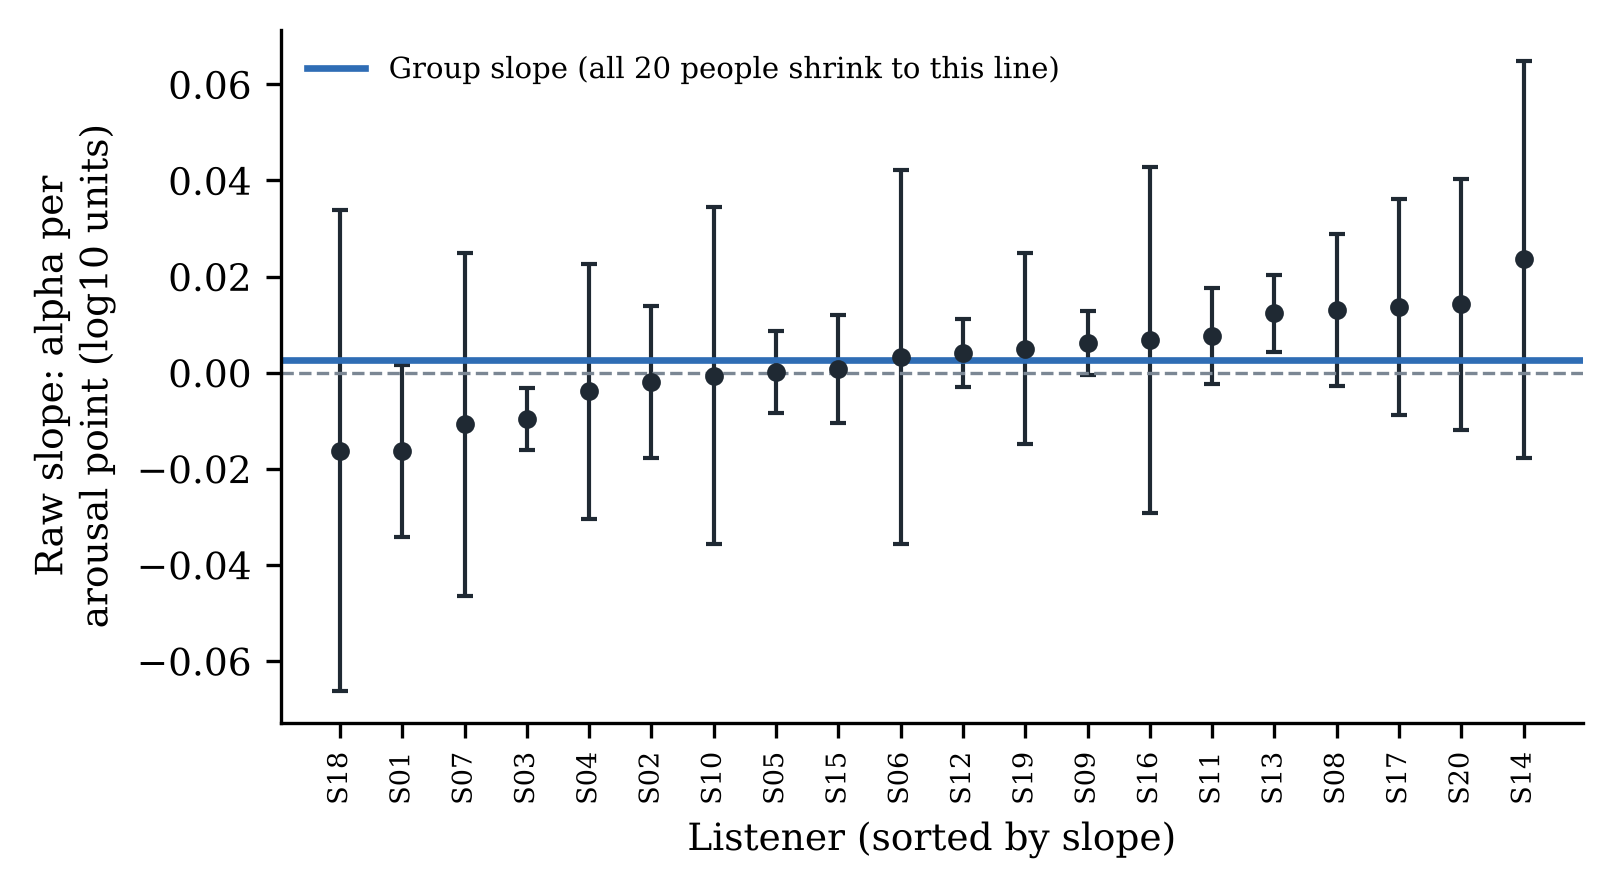
\includegraphics[width=0.68\linewidth]{figures/fig5_person_slopes.png}
\caption{Each listener's own slope of posterior alpha on arousal, with a 95\% interval. The spread is what random noise from about 20 songs per person would produce; the model shrinks every listener onto the blue group line.}
\label{fig:slopes}
\end{figure}

\subsection{Casting a wider net}

Perhaps the classic markers are simply the wrong place to look. The exploratory grid searched every combination of five bands, seven regions and three ratings (Figure~\ref{fig:grid}). Three of the 105 tests had uncorrected $p < .05$: alpha and beta over central sites with arousal, and gamma over the right temporal region with valence. By chance alone, about five would be expected. None survived the false discovery rate correction; the smallest corrected value was $q = 0.996$. The right temporal gamma result is also the kind most likely to reflect muscle tension rather than brain activity. These are ideas for a future study, not findings.

\begin{figure}[!htb]
\centering
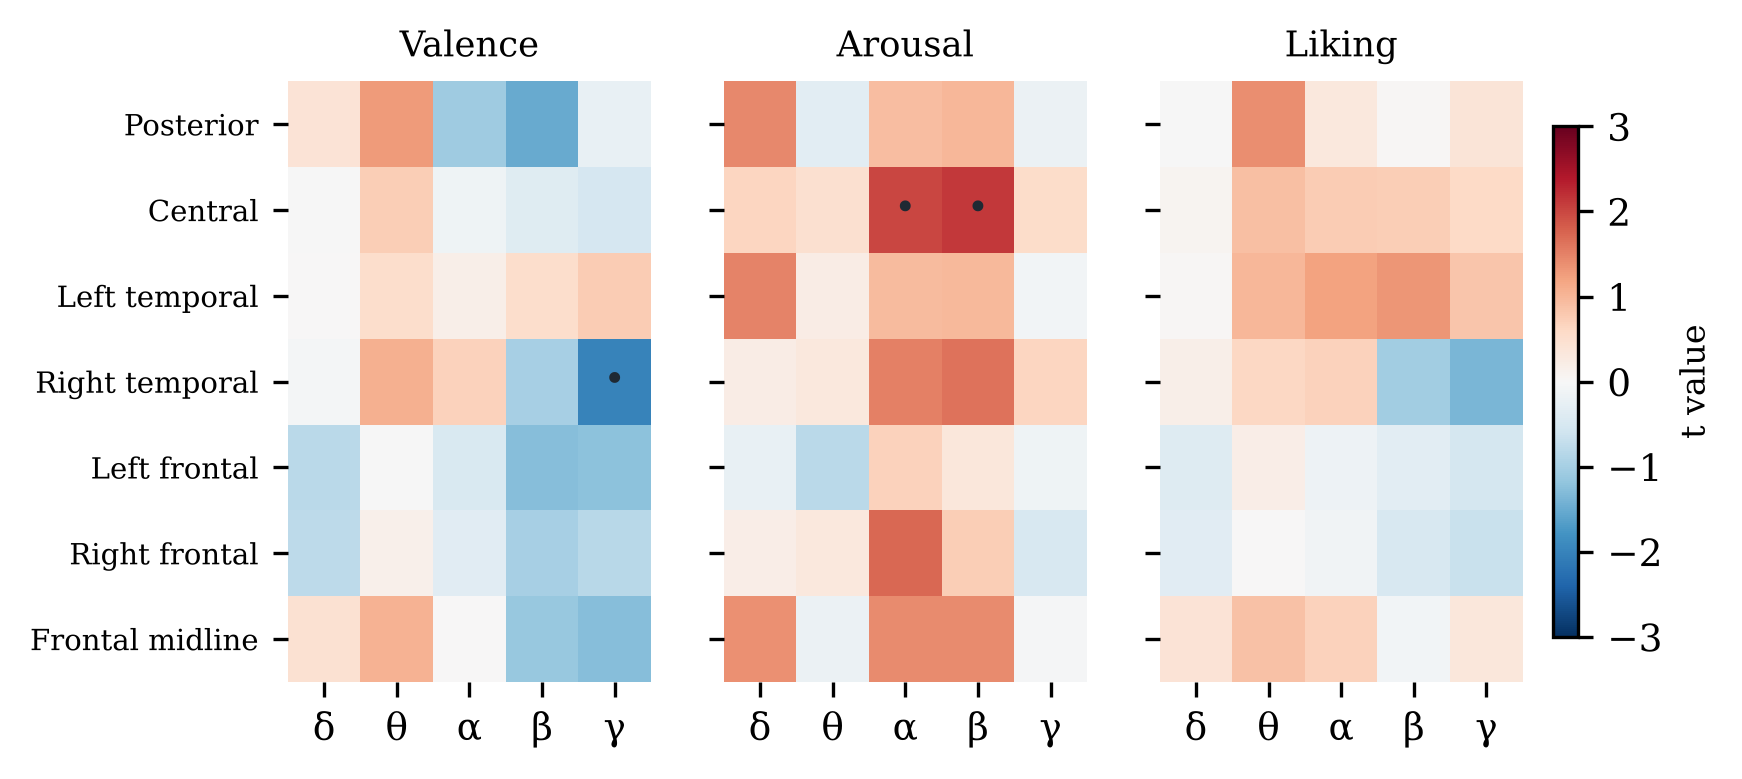
\includegraphics[width=0.82\linewidth]{figures/fig6_exploratory.png}
\caption{The exploratory grid of 105 tests. Colour shows the $t$ value of each within person slope; dots mark uncorrected $p < .05$. The pattern is what chance produces: a few pale spots and nothing that survives correction.}
\label{fig:grid}
\end{figure}

\subsection{Pushing on the result}

A finding that depends on one arbitrary decision is fragile. The null result here did not depend on any. Across the four alternative analyses in Figure~\ref{fig:forest}, the standardized H1 slope ranged from 0.03 to 0.06 (all $p > .25$) and the H2 slope from \m0.01 to 0.05 (all $p > .50$). Leaving out each listener in turn moved the raw H1 slope only between 0.0016 and 0.0037, and the H2 slope between \m0.0015 and 0.0028, so no single person drove the outcome. Residual diagnostics showed no serious departures from the model's assumptions.

\section{Discussion}

\subsection{What a careful null tells us}

The story this study set out to tell was simple: when a song moves you more than it moves others, your brain rhythms should show it. The data did not tell that story. Neither posterior alpha nor frontal alpha asymmetry tracked how aroused or how pleased a listener felt relative to their own usual ratings, and the person specific part of the experience showed no trace either. Listeners did not appear to differ in these relationships, and a broad exploratory search found nothing beyond chance.

A non significant result is not proof of no effect, but these results are more informative than a bare ``not significant'', because the confidence intervals are narrow (Lakens, 2017). For H1, the interval from \m0.05 to 0.15 means that a one standard deviation increase in a person's felt arousal is unlikely to lower their posterior alpha by more than about a twentieth of its within person variation. For H2, effects larger than about 0.11 standard deviations in either direction are unlikely. If these relationships exist at the level of whole songs, they are small.

\subsection{Why might classic effects vanish here?}

These results sit uneasily with the textbook picture in which alpha tracks arousal and frontal asymmetry tracks pleasure (Klimesch, 1999; Davidson, 1992), and with music studies that reported asymmetry for joyful versus sad excerpts (Schmidt \& Trainor, 2001). Three differences in design may explain the gap.

First, \textbf{the comparison is different}. Earlier evidence mostly compared stimuli or conditions, where acoustics, attention and expectation all differ. This study removed those differences by holding the song constant and looking only at personal variation. If much of the classic effect was carried by the stimulus, it is not surprising that little remains once the stimulus is held fixed.

Second, \textbf{the timescale is coarse}. Each EEG value averages two full minutes, and each rating is a single judgement given after the music ended. Musical emotion unfolds in moments: a chord change, a climax, a voice entering. A response lasting a few seconds would be diluted almost to nothing in a 120 second average, and a single retrospective rating cannot say when the feeling occurred.

Third, \textbf{the signal is small relative to the noise}. Ninety four percent of the variance in posterior alpha was between people. Whatever emotion did within a person had to compete with song to song fluctuations in alertness, fatigue and attention, all of which also move alpha. And the valence manipulation was weak: with no truly unpleasant songs, the range over which valence could act was narrow.

\subsection{What this study does not show}

Two cautions keep the interpretation honest. The first concerns reverse inference (Poldrack, 2006). Even if alpha had fallen with arousal, lower alpha would not show that a person felt aroused, because alertness, visual attention and many other states lower alpha too. A null result guards against this error by default, but the same caution applies to any positive finding from the exploratory grid. The second concerns causation. Ratings were given after each song and the EEG was averaged across it, so the design is correlational; neither variable was manipulated to cause the other.

Nor does this study show that EEG is blind to musical emotion. It shows that two specific, widely cited alpha markers, measured over whole songs in twenty people, did not follow personal emotional experience. That is a narrower and more useful conclusion.

\subsection{Limitations}

The sample was small (20 listeners and 20 songs), which limits the precision of individual slopes and is typical of the power problems in neuroscience more broadly (Button et al., 2013). The design offered one retrospective rating per two minute excerpt, a compressed valence range and an assumed music onset. Preprocessing was partly inherited and partly undocumented, no independent component analysis was rerun, and flagged channels were dropped rather than interpolated. Scalp EEG cannot see deep emotional circuitry and is blurred by volume conduction. The ratings are ordinal but were treated as numeric. Presentation order could not be recovered, so order and fatigue effects remain uncontrolled. Finally, one recording was truncated and one was missing in the published data. Each of these could hide a smaller or more time specific effect.

\subsection{What comes next}

The results point clearly to the next experiment. Continuous ratings, collected with a slider while the music plays, would allow the EEG to be aligned with moments of feeling rather than averaged across whole songs. Time resolved analyses could then ask whether alpha or asymmetry shifts in the seconds around a peak of emotion. More songs per listener would sharpen each person's slope and make it possible to learn whether people truly differ. A song set that includes genuinely unpleasant music would widen the valence range. And because the consensus and deviation split worked as intended, it could be reused in any such design to keep the song and the self apart.

\section{Conclusion}

Twenty listeners each heard the same twenty songs, and I asked whether their brain rhythms followed what they personally felt. After a plan written down in advance, a careful cleaning of the data and a battery of checks, the answer was no detectable link. Posterior alpha did not fall when a person felt more aroused than usual, frontal asymmetry did not rise when a person felt more pleased than usual, and the part of the feeling unique to each listener left no visible trace. The narrow confidence intervals make large effects of this kind unlikely. The song, it seems, is easy to find in the ratings; the self is much harder to find in the alpha rhythm. Finding it will take measures that move as fast as music does.

\section*{Data and code availability}

The data are publicly available from OpenNeuro (dataset ds008701, version 1.0.4). All analysis code, the preregistration with its commit history, every result table and the scripts that produced the figures in this paper are available in the author's public GitHub repository (account Koundinya2003). The preregistration was committed on 6 October 2026 at 15:27 IST, before the statistics script was run, and has not been edited since. Three deviations from it are reported above: the singular fit fallback to random intercepts, the presentation order analysis that could not be run, and the slope SD intervals that could not be estimated.

\section*{References}
\small
\setlength{\parindent}{0pt}
\setlength{\parskip}{0.3em}
\everypar{\hangindent=1.5em \hangafter=1}

Allen, J. J. B., Coan, J. A., \& Nazarian, M. (2004). Issues and assumptions on the road from raw signals to metrics of frontal EEG asymmetry in emotion. \emph{Biological Psychology, 67}(1, 2), 183 to 218.

Barr, D. J., Levy, R., Scheepers, C., \& Tily, H. J. (2013). Random effects structure for confirmatory hypothesis testing: Keep it maximal. \emph{Journal of Memory and Language, 68}(3), 255 to 278.

Barry, R. J., Clarke, A. R., Johnstone, S. J., Magee, C. A., \& Rushby, J. A. (2007). EEG differences between eyes closed and eyes open resting conditions. \emph{Clinical Neurophysiology, 118}(12), 2765 to 2773.

Bates, D., M\"achler, M., Bolker, B., \& Walker, S. (2015). Fitting linear mixed effects models using lme4. \emph{Journal of Statistical Software, 67}(1), 1 to 48.

Benjamini, Y., \& Hochberg, Y. (1995). Controlling the false discovery rate: A practical and powerful approach to multiple testing. \emph{Journal of the Royal Statistical Society: Series B, 57}(1), 289 to 300.

Bradley, M. M., \& Lang, P. J. (1994). Measuring emotion: The Self Assessment Manikin and the semantic differential. \emph{Journal of Behavior Therapy and Experimental Psychiatry, 25}(1), 49 to 59.

Button, K. S., Ioannidis, J. P. A., Mokrysz, C., Nosek, B. A., Flint, J., Robinson, E. S. J., \& Munaf\`o, M. R. (2013). Power failure: Why small sample size undermines the reliability of neuroscience. \emph{Nature Reviews Neuroscience, 14}(5), 365 to 376.

Cheang, W. L. (2026). \emph{MET: Music Induced EEG Dataset} (Version 1.0.4) [Data set]. OpenNeuro. \url{https://doi.org/10.18112/openneuro.ds008701.v1.0.4}

Coan, J. A., \& Allen, J. J. B. (2004). Frontal EEG asymmetry as a moderator and mediator of emotion. \emph{Biological Psychology, 67}(1, 2), 7 to 49.

Davidson, R. J. (1992). Emotion and affective style: Hemispheric substrates. \emph{Psychological Science, 3}(1), 39 to 43.

Hurlbert, S. H. (1984). Pseudoreplication and the design of ecological field experiments. \emph{Ecological Monographs, 54}(2), 187 to 211.

Juslin, P. N., \& V\"astfj\"all, D. (2008). Emotional responses to music: The need to consider underlying mechanisms. \emph{Behavioral and Brain Sciences, 31}(5), 559 to 575.

Klimesch, W. (1999). EEG alpha and theta oscillations reflect cognitive and memory performance: A review and analysis. \emph{Brain Research Reviews, 29}(2, 3), 169 to 195.

Kuznetsova, A., Brockhoff, P. B., \& Christensen, R. H. B. (2017). lmerTest package: Tests in linear mixed effects models. \emph{Journal of Statistical Software, 82}(13), 1 to 26.

Lakens, D. (2017). Equivalence tests: A practical primer for t tests, correlations, and meta analyses. \emph{Social Psychological and Personality Science, 8}(4), 355 to 362.

Muthukumaraswamy, S. D. (2013). High frequency brain activity and muscle artifacts in MEG/EEG: A review and recommendations. \emph{Frontiers in Human Neuroscience, 7}, 138.

Nosek, B. A., Ebersole, C. R., DeHaven, A. C., \& Mellor, D. T. (2018). The preregistration revolution. \emph{Proceedings of the National Academy of Sciences, 115}(11), 2600 to 2606.

Poldrack, R. A. (2006). Can cognitive processes be inferred from neuroimaging data? \emph{Trends in Cognitive Sciences, 10}(2), 59 to 63.

Reznik, S. J., \& Allen, J. J. B. (2018). Frontal asymmetry as a mediator and moderator of emotion: An updated review. \emph{Psychophysiology, 55}(1), e12965.

Russell, J. A. (1980). A circumplex model of affect. \emph{Journal of Personality and Social Psychology, 39}(6), 1161 to 1178.

Schmidt, L. A., \& Trainor, L. J. (2001). Frontal brain electrical activity (EEG) distinguishes valence and intensity of musical emotions. \emph{Cognition and Emotion, 15}(4), 487 to 500.

Self, S. G., \& Liang, K. Y. (1987). Asymptotic properties of maximum likelihood estimators and likelihood ratio tests under nonstandard conditions. \emph{Journal of the American Statistical Association, 82}(398), 605 to 610.

Welch, P. (1967). The use of fast Fourier transform for the estimation of power spectra: A method based on time averaging over short, modified periodograms. \emph{IEEE Transactions on Audio and Electroacoustics, 15}(2), 70 to 73.

\end{document}
